\documentclass[9pt,twocolumn,twoside]{pnas-new}
% Use the lineno option to display guide line numbers if required.
% twocolumn

\templatetype{pnasresearcharticle} % Choose template 
% {pnasresearcharticle} = Template for a two-column research article
% {pnasmathematics} %= Template for a one-column mathematics article
% {pnasinvited} %= Template for a PNAS invited submission

\title{\emph{Skew}DB: A comprehensive database of GC and a dozen other skews for over 23,000 chromosomes}

% Use letters for affiliations, numbers to show equal authorship (if applicable) and to indicate the corresponding author
\author[a]{Bert Hubert}
%\affil[a]{Independent}

% Please give the surname of the lead author for the running footer
\leadauthor{Hubert} 

% Please add here a significance statement to explain the relevance of your work
\significancestatement{GC and TA skew are small ($\pm2.5\%$) deviations in nucleotide frequencies between the leading and lagging replication strands of eubacteria. These deviations show patterns within and across phyla, thus highlighting differences between superficially similar organisms. Such differences may guide research into bacterial replication mechanisms. This work describes a database with details of many skews for over 23,000 bacterial chromosomes.}

% Please include corresponding author, author contribution and author declaration information
%\authorcontributions{Please provide details of author contributions here.}
%\authordeclaration{Please declare any conflict of interest here.}
%\equalauthors{\textsuperscript{1}A.O.(Author One) and A.T. (Author Two) contributed equally to this work (remove if not applicable).}
\correspondingauthor{\textsuperscript{a}To whom correspondence should be addressed. E-mail: bert@hubertnet.nl}

% Keywords are not mandatory, but authors are strongly encouraged to provide them. If provided, please include two to five keywords, separated by the pipe symbol, e.g:
\keywords{GC skew $|$ TA skew $|$ strand bias $|$ codon bias} 

\begin{abstract}
  GC skew \cite{lobry_asymmetric_1996} denotes the relative excess of G nucleotides over C nucleotides on the leading versus the lagging replication strand of eubacteria. While small, typically around 2.5\%, the effect is robust and pervasive, showing up in almost all circular chromosomes. GC skew and the analogous TA skew are a localized deviation from Chargaff's second parity rule \cite{rudner_separation_1968}, which states that G and C, and T and A occur with (mostly) equal frequency even within a strand.

  Unlike archaea, bacteria show very well defined GC skew, often highly stable over the entire leading and lagging strands. The excess of G on the leading strand is on average negated by the excess of C on the lagging strand.

  Most bacteria also show the analogous TA skew, although this is often noisier than GC skew, with more local deviations. Different phyla show different relations between TA and GC skew \cite{charneski_atypical_2011}.

  This article introduces a database (\url{https://skewdb.org}) of GC and 12 other skews for over 23,000 chromosomes. Many other details like codon bias, strand bias, strand lengths and taxonomic data are also included. The \emph{Skew}DB database can be used to generate or verify hypotheses. Since the origins of both the second parity rule, as well as GC skew itself, are not yet satisfactorily explained, such a database may enhance our understanding of microbial DNA.

  In this work various interesting chromosomes are highlighted which show asymmetric skews and strands, or other hard to explain phenomena. I also show how GC skew is an interesting forensic tool for studying DNA assembly problems, but also possible chromosome or plasmid mergers, which show up clearly in the graphs generated using the \emph{Skew}DB. 
\end{abstract}

\dates{This manuscript was compiled on \today}
\doi{\url{www.berthub.eu/cgi/doi/10.1073/bhub.XXXXXXXXXX}}

\begin{document}

\maketitle
\thispagestyle{firststyle}
\ifthenelse{\boolean{shortarticle}}{\ifthenelse{\boolean{singlecolumn}}{\abscontentformatted}{\abscontent}}{}

The phenomenon of GC skew is tantalizing because it enables a simple numerical analysis that accurately predicts the loci of both the origin and terminus of replication in most bacteria \cite{lu_skewit_2020} \cite{luo_doric_2019}.

Bacterial DNA is typically replicated simultaneously on both strands, starting at the origin of replication. Both copying forks (naturally) travel in the 5' to 3' direction, but given that the replichores are on opposite strands, topologically they are traveling in opposite directions. This continues until the forks meet again at the terminus.

The excess of G over C on the leading strand is in itself only remarkable because of Chargaff's somewhat mysterious second parity rule, which states that within a DNA strand, there are near equal numbers of G's and C's, and similarly, T's and A's. This rule does not directly follow from the first parity rule, which is a simple statement of base pairing rules.

Depending on who is asked, Chargaff's second parity rule is so trivial that it needs no explanation, or it requires complex mathematics and entropy considerations to explain its existence \cite{fariselli_dna_2020}.

The origins of GC skew are still being debated. The leading and lagging strands of circular bacterial chromosomes are replicated very differently; it is at least plausible that this leads to different mutational biases. In addition, there are selection biases that are theorized to be involved \cite{tillier_contributions_2000}. No single mechanism may be exclusively responsible.

This article does not attempt to explain or further mystify \cite{zhang_brief_2014} the second parity rule or GC skew, but it may be that the contents of the \emph{Skew}DB might contribute to our further understanding.

The \emph{Skew}DB also contains hard to explain data on many chromosomes. These include highly asymmetric skew, but also very disparate strand lengths. On the positive side, the \emph{Skew}DB confirms earlier work on skews in the Firmicute phylum  \cite{charneski_atypical_2011}, and also expands on these earlier findings.

GC skew has often been investigated by looking at windows of DNA of a certain size. It has been found that this chosen size impacts the results of the analysis. In what follows, I only look at cumulative skew \cite{grigoriev_analyzing_1998}. This sidesteps window size issues. For example, the sequence GGGCCC has a cumulative GC skew of zero. However, as we progress through the sequence, this skew takes on values 0, 1, 2, 3, 2, 1, 0.

The result of such an analysis is shown in figure \ref{fig:explainer-graph}. The analysis software fits a linear model on the skews, where it also compensates for chromosome files sequenced in the non-canonical direction, or where the origin of replication is not at the start of the file.

\section*{\emph{Skew}DB: GC and TA skew across 23,725 chromosomes}
Using simple statistical techniques and open source software, I analysed 23,725 chromosomes for their GC, TA and other skews.
These chromosomes have been sourced from the NCBI download service. Using the associated annotation data (GFF3), the skews are also reported split out over the first, second and third codon positions, and also for non-coding regions.

In addition, the analysis also includes statistics on codon bias and strand bias (the phenomenon where genes tend to reside more on the leading replication strand). To make life easier, the database also features further statistics on GC-percentage, as well as taxonomic details.

The statistical model also captures interesting asymmetries. Although no plausible mechanism is known, some chromosomes feature very different GC skews between leading and lagging strands. Similarly, some strands appear to differ in length by whole factors, something which would negatively impact chromosome replication speed.

To prevent plasmids from skewing the numbers, only chromosomes of 1 million nucleotides or more are included. 

The \emph{Skew}DB software (``Antonie'') is fully open source. The generation of the database requires a few hours of CPU time. More information on the software and how to recreate the database are described in the methods section.

\section*{What is in the database}
The \emph{Skew}DB contains several kinds of data. First for each chromosome there are raw counts of nucleotides, also split out by codon position, coding sense and coding status. These numbers are provided with 4096-nucleotide resolution, as well as whole-chromosome totals. From these counts, detailed graphs can be generated per chromosome.

At one level higher, all the skews are summarised down to three biologically relevant parameters which describe the skews on the leading and lagging replication strands, plus the relative length of these strands. A goodness-of-fit parameter (relative RMS) is also provided. This parameter is not only for quality assurance, it also reliably spots exotic or anomalous chromosomes.

For each chromosome, codon bias data is also included. Finally for ease of processing, taxonomic data is sourced and merged, enabling the creation of per phylum or other phylogenetic demarcations. 

\section*{Skew details}

\begin{figure}[ht]
\centering
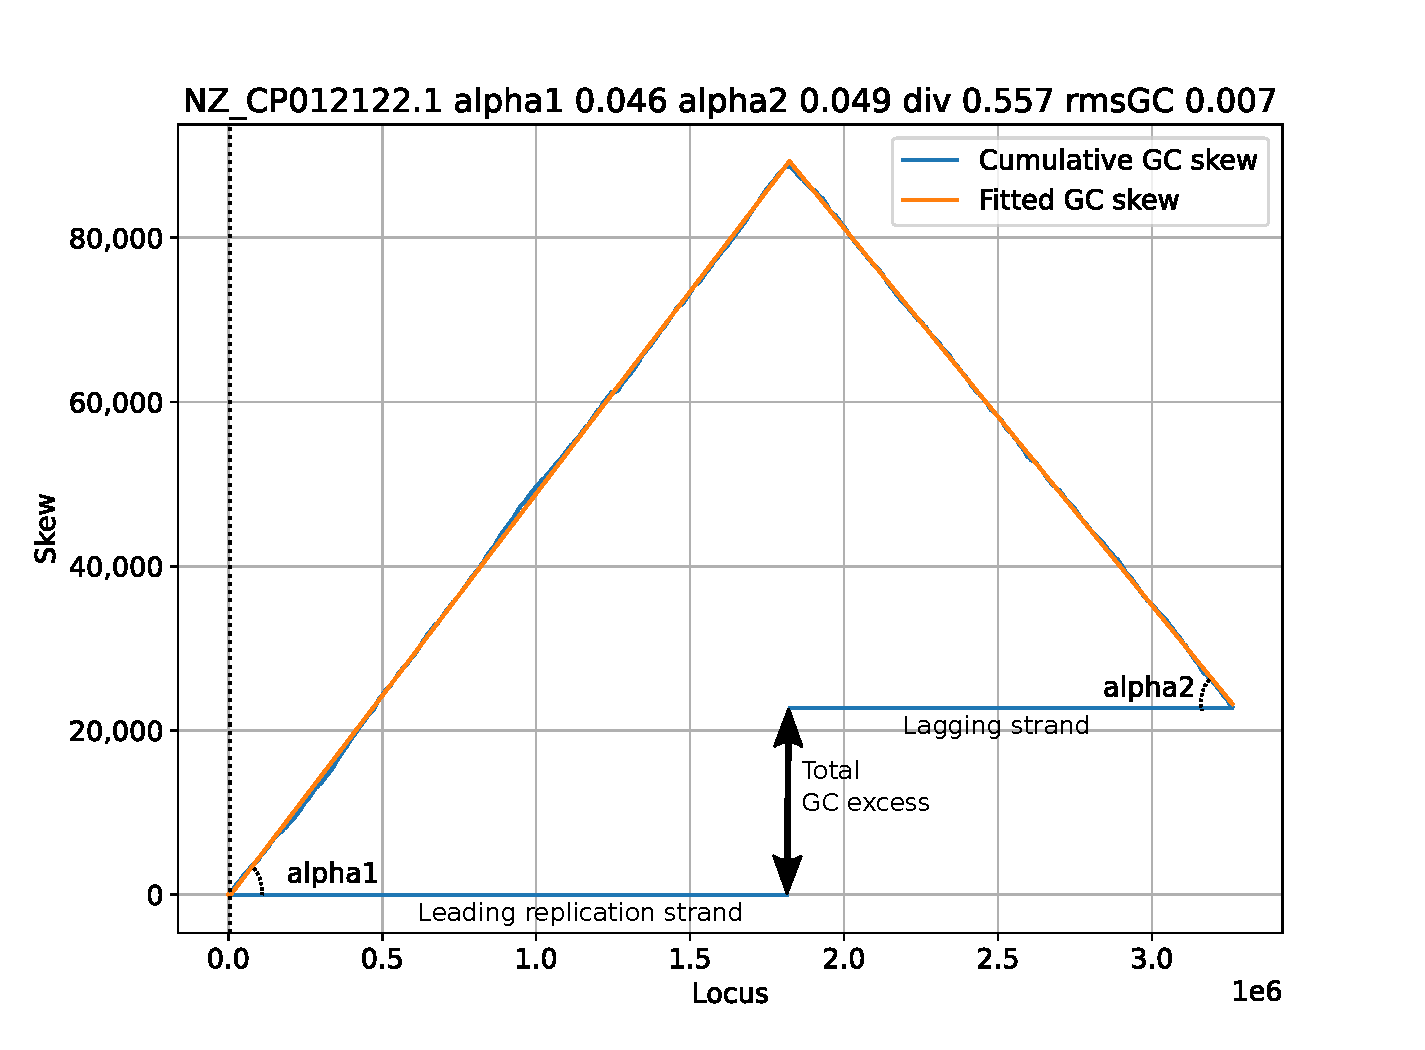
\includegraphics[width=.9\linewidth]{explainer.pdf}
\caption{Sample graph showing \emph{Skew}DB data for Lactiplantibacillus plantarum strain LZ95 chromosome}
\label{fig:explainer-graph}
\end{figure}

The fits are based on four parameters, as shown in figure \ref{fig:explainer-graph}. {\tt Alpha1} and {\tt alpha2} denote the relative excess of G over C on the leading and lagging strands. If {\tt alpha1} is $0.046$, this means that for every 1000 nucleotides on the leading strand, the cumulative count of G excess increases by 46.

The third parameter is {\tt div} and it describes how the chromosome is divided over leading and lagging strands. If this number is $0.557$, the leading replication strand is modeled to make up $55.7\%$ of the chromosome.

The final parameter is {\tt shift} (the dotted vertical line), and denotes the offset of the origin of replication compared to the DNA FASTA file. This parameter has no biological meaning, and is an artifact of the DNA assembly process. 

The goodness-of-fit number consists of the root mean squared error of the fit, divided by the absolute mean skew. This latter correction is made to not penalize good fits for bacteria showing significant skew.

Both GC and TA skews are reported, for the whole genome, but also split out on first, second or third codon positions. In addition, separate numbers are included for non-genomic and genomic skews. Finally, a ``strand bias'' skew is reported, in which each positive sense nucleotide counts upwards, and each anti-sense nucleotide counts down.

Exhaustive details on all the metrics can be found on \url{https://skewdb.org}. This also includes links to a Jupyter \cite{Kluyver:2016aa} notebook that uses Matplotlib \cite{Hunter:2007} and Pandas \cite{jeff_reback_2021_5203279} to create all the graphs from this article, and many more. In addition, this notebook shows all numerical claims made in this work.

\section*{Sample findings}
In what follows, I discuss some findings that can trivially be extracted from the \emph{Skew}DB. 

\subsection*{GC and TA skews}
Most bacteria show concordant GC and TA skew, with an excess of G correlating with an excess of T. This does not need to be the case however. Figure \ref{fig:gc-ta-scatter} is a scatterplot that shows the correlation between the skews for various major superphyla. Firmicutes (part of the Terrabacteria group) show clearly discordant skews.
\begin{figure}[ht]
\centering
\includegraphics[width=.9\linewidth]{phylo-histo.png}
\caption{Scatter graph of 25,000 chromosomes by superphylum, GC skew versus TA skew}
\label{fig:gc-ta-scatter}
\end{figure}

\subsection*{Firmicute prediction}
In many bacteria, genes tend to concentrate on the leading replication strand. If the codon bias of genes is such that they are relatively rich in one nucleotide, the ``strand bias'' may itself give rise to GC or TA bias. Or in other words, if genes contain a lot of G's and they huddle on the leading strand, that strand will show GC skew. As an hypothesis, we can plot the observed GC and TA skews for all Firmicutes for which we have data.

\begin{figure}[ht]
\centering
\includegraphics[width=.9\linewidth]{firmi.pdf}
\caption{Predicted versus actual GC/TA skew for 4093 Firmicutes}
\label{fig:the-big-graph}
\end{figure}


Mathematically the relation between the codon bias, strand bias and predicted GC skew turns out to be a simple multiplication. In figure \ref{fig:the-big-graph}, the x-axis represents this multiplication. The y-axis represents the GC and TA skew ratio. 

It can clearly be seen that both GC and TA skew correlate strongly with the codon/strand bias product. TA skew goes to zero with the two biases, but GC skew appears to persist even in the absence of such biases.

\begin{figure}[ht]
\centering
\includegraphics[width=.9\linewidth]{cdif-histo.pdf}
\caption{Scatter graph of codon/strand bias versus GC/TA skew for C. difficile}
\label{fig:cdif-scatter}
\end{figure}


Figure \ref{fig:cdif-scatter} shows the situation for an individual chromosome (C. difficile), based on overlapping 40960-nucleotide segments. On the x-axis we find the strand bias for these segments, running from entirely negative sense genes to entirely positive sense genes. The skew is meanwhile plotted on the y-axis, and here too we see that TA skew goes to zero in the absence of strand bias, while GC skew persists and clearly has an independent strand-based component.

\subsection*{Asymmetric skew}
The vast majority of chromosomes show similar skews on the leading and the lagging replication strands, something that makes sense given the pairing rules. There are however many chromosomes that have very asymmetric skews, with one strand sometimes showing no skew at all. In figure \ref{fig:asym-skew} four chromosomes are shown that exhibit such behavior. The \emph{Skew}DB lists around 250 chromosomes where one strand shows a GC skew at least 3 times bigger/smaller than the other one.

\begin{figure}[ht]
\centering
\includegraphics[width=.9\linewidth]{flat-skew.pdf}
\caption{Chromosomes with asymmetric skews}
\label{fig:asym-skew}
\end{figure}


\subsection*{Asymmetric strands}
Bacteria tend to have very equally sized replication strands, which is also an optimum for the duration of replication. It is therefore interesting to observe that GC skew analysis finds many chromosomes where one strand is four times larger than the other strand.  In  figure \ref{fig:strand-div} four such chromosomes are shown. The \emph{Skew}DB lists around 100 chromosomes where one strand is at least three times as large as the other strand.
\begin{figure}[ht]
\centering
\includegraphics[width=.9\linewidth]{strand-div.pdf}
\caption{Chromosomes with differing strand lengths}
\label{fig:strand-div}
\end{figure}


\subsection*{Anomalies}
In many ways, GC skew is like a forensic record of the historical developments in a chromosome. Horizontal gene transfer, inversions, integration of plasmids, excisions can all leave traces. In addition, DNA sequencing or assembly artifacts will also reliably show up in GC graphs.

Figure \ref{fig:anomalous} shows the GC and TA skews for Salmonella enterica subsp. enterica serovar Concord strain AR-0407 (NZ\_CP044177.1), and many things could be going on here. The peaks might correspond to multiple origins of replication, but might also indicate inversions or DNA assembly problems.

To find such anomalies, the \emph{Skew}DB viewer (\url{https://skewdb.org/view}) offers various buttons to show random anomalous chromosomes. 

\begin{figure}[ht]
\centering
\includegraphics[width=.9\linewidth]{anomalous.pdf}
\caption{GC and TA skew for Salmonella enterica subsp. enterica serovar Concord strain AR-0407}
\label{fig:anomalous}
\end{figure}

\section*{Limitations and quality}
The existential limitation of any database like the \emph{Skew}DB is that it does not represent nature. The sequence and annotation databases are dominated by easily culturable microbes. And even within that selection, specific (model) bacteria are heavily oversampled because of their economic or medical relevance.

Because of this, care should be taken not to interpret numbers in a way that does not take such over- and undersampling into account. This leaves enough room however for finding correlations. Some metrics are sampled so heavily that it would be a miracle if the unculturable organisms were collectively conspiring to skew the statistics away from what we are seeing.

The \emph{Skew}DB fits skews to a relatively simple model of only three parameters. This prevents overfitting, and this model has proven to be robust in practice. Yet, when doing automated analysis of tens of thousands of chromosomes, mistakes will be made. 

\begin{figure}[tbhp]
\centering
\includegraphics[width=.9\linewidth]{rms-samples.pdf}
\caption{\emph{Skew}DB fits for 16 equal sized quality categories}
\label{fig:rms-samples}
\end{figure}

Figure \ref{fig:rms-samples} shows 16 equal sized quality categories, where it is visually clear that the 88\% best fits are excellent. It is therefore reasonable to filter the database on $RMS_{gc}<0.1067$. Or conversely, above that limit, interesting anomalous chromosomes can be found.

\section*{Discussion}
Chargaff's second parity rule, GC and other skews are still open to further research. Previously, no database was available that covers such a wide variety of skews and genomes.

The \emph{Skew}DB is aimed at biologists so they can use the data to generate or even reject hypotheses. In addition, it may be that by going through the chromosomes with anomalous skews, badly assembled sequences can be detected and removed or redone.

Nucleotide skews, especially when split out by codon position, coding status and strand, may be able to tell us more about microbiology than previously thought, especially given that such a robust effect remains at best partially explained.

Specifically, given the abundance of data found in the \emph{Skew}DB, it may be possible to use statistics to constrain the possible origins of the various skews. If GC skew is truly a random process, the resulting distribution of skews can be calculated from first principles and compared to the biological reality.

\matmethods{All software and processes to generate the \emph{Skew}DB are open source. The source code can be found through \url{https://skewdb.org}, where details are also available how to rebuild the database. All annotations and sequences are obtained from the NCBI download service. The software is also described in XXX.}

\showmatmethods{} % Display the Materials and Methods section

\acknow{I would like to thank Bertus Beaumont for helping me to think like a biologist, and Jason Piper for regularly pointing me to the relevant literature. In addition, I am grateful that Felix Hol kindly allowed me to field test my software on his DNA sequences \cite{hol_density-dependent_2016}.}

\showacknow{} % Display the acknowledgments section

% Bibliography
\bibliography{references}

\end{document}
